
        \documentclass[addpoints,spanish, 12pt,a4paper]{exam}
        %\documentclass[answers, spanish, 12pt,a4paper]{exam}
        % \printanswers
        
        \pointpoints{punto}{puntos}
        \hpword{Puntos:}
        \vpword{Puntos:}
        \htword{Total}
        \vtword{Total}
        \hsword{Resultado:}
        \hqword{Ejercicio:}
        \vqword{Ejercicio:}

        \usepackage[utf8]{inputenc}
        \usepackage[spanish]{babel}
        \usepackage{eurosym}
        %\usepackage[spanish,es-lcroman, es-tabla, es-noshorthands]{babel}


        \usepackage[margin=1in]{geometry}
        \usepackage{amsmath,amssymb}
        \usepackage{multicol, xparse}

        \usepackage{yhmath}

        \usepackage{verbatim}
        %\usepackage{pstricks}


        \usepackage{graphicx}
        \graphicspath{{../img/}}




        \let\multicolmulticols\multicols
        \let\endmulticolmulticols\endmulticols
        \RenewDocumentEnvironment{multicols}{mO{}}
         {%
          \ifnum#1=1
            #2%
          \else % More than 1 column
            \multicolmulticols{#1}[#2]
          \fi
         }
         {%
          \ifnum#1=1
          \else % More than 1 column
            \endmulticolmulticols
          \fi
         }
        \renewcommand{\solutiontitle}{\noindent\textbf{Sol:}\enspace}

        \newcommand{\samedir}{\mathbin{\!/\mkern-5mu/\!}}

        \newcommand{\class}{1º Bachillerato}
        \newcommand{\examdate}{\today}

        %\newcommand{\tipo}{A}


        \newcommand{\timelimit}{80 minutos}

        \renewcommand{\solutiontitle}{\noindent\textbf{Solución:}\enspace}


        \pagestyle{head}
        \firstpageheader{
\includegraphics[width=0.2\columnwidth]{header_left}}{\textbf{Departamento de Matemáticas\linebreak \class}\linebreak \examnum}{
\includegraphics[width=0.1\columnwidth]{header_right}}
        \runningheader{\class}{\examnum}{Página \thepage\ of \numpages}
        \runningheadrule
        
        \pointsinrightmargin % Para poner las puntuaciones a la derecha. Se puede cambiar. Si se comenta, sale a la izquierda.
        \extrawidth{-2.4cm} %Un poquito más de margen por si ponemos textos largos.
        \marginpointname{ \emph{\points}}

        
            \newcommand{\tipo}{A}\newcommand{\examnum}{Examen Global}
        \begin{document}
        \noindent
        \begin{tabular*}{\textwidth}{l @{\extracolsep{\fill}} r @{\extracolsep{6pt}} }
        \textbf{Nombre:} \makebox[3.5in]{\hrulefill} & \textbf{Fecha:}\makebox[1in]{\hrulefill} \\
        & \\
        \textbf{Tiempo: \timelimit} & Tipo: \tipo 
        \end{tabular*}
        \rule[2ex]{\textwidth}{2pt}
%        Esta prueba tiene \numquestions\ ejercicios. La puntuación máxima es de \numpoints. 
%        La nota final de la prueba será la parte proporcional de la puntuación obtenida sobre la puntuación máxima. 
\begin{center}
\rule[2ex]{\textwidth}{2pt}        
\textbf{Instrucciones:} \begin{itemize}
\item \textbf{Si solo tienes una evaluación pendiente:} Tienes que hacer \textbf{todos} los ejercicios del bloque correspondiente a la evaluación, incluido el "postre". (4 ejercicios en total). \textbf{Tiempo: 50 minutos}
\item \textbf{Si tienes más de una pendiente:} Tienes que hacer \textbf{los dos primeros} ejercicios de cada evaluación. (6 ejercicios en total). \textbf{Tiempo: 75 minutos}
\item \textbf{Si tienes todo aprobado} tienes que hacer de cada evaluación el \textbf{último ejercicio o ejercicio "postre"} y otro a elegir \textbf{entre los dos primeros}. (6 ejercicios en total) \textbf{Tiempo: 75 minutos}
\end{itemize}
\rule[2ex]{\textwidth}{2pt}
\end{center}



        
        
        
% \rule[2ex]{\textwidth}{2pt}
%       
%        \begin{center}
%
%
%        \addpoints
%             %\gradetable[h][questions]
%            \pointtable[h][questions]
%        \end{center}
%
%        \noindent
% \rule[2ex]{\textwidth}{2pt}

        \begin{questions}

%        \question Calcula los siguientes límites:
%        \begin{multicols}{1}
%        \begin{parts} \part[1] $$\lim_{x \to 3}\left(\frac{3 x^{2} - 11 x + 6}{x^{3} - 3 x^{2} + x - 3}\right)$$  \begin{solution}   $\frac{7}{10}$   \end{solution} \part[1] $$\lim_{x \to \infty} e^{1 - x}$$  \begin{solution}   $0$   \end{solution} \part[1] $$\lim_{x \to -2}\left(\frac{x^{3} + x^{2} - x + 2}{x^{2} + 4 x + 4}\right)$$  \begin{solution}   No existe el límite   \end{solution} \part[2] $$\lim_{x \to 2} \left(\frac{x^{3} - 4}{x^{2}}\right)^{\frac{1}{x - 2}}$$  \begin{solution}   $e^{2}$   \end{solution}
%        \end{parts}
%        \end{multicols}
\section*{1ª Evaluación}        
        \question[1] Resuelve:
        \begin{multicols}{2}
        \begin{parts} \part $$\left\{ 					\begin{gathered}
	  		\log_{y}{(9-x)}=\frac{1}{2} \hfill \\
	  		\log_{x}{(y+9)}=2 \hfill \\ 
	\end{gathered}  \right.$$  \begin{solution}   $(5,16)$   \end{solution}
		 \part $\sqrt{3x+10}-2=\sqrt{15x+6}$  \begin{solution}   $-\frac{1}{3}$, 2 NO   \end{solution}
		 \part $\dfrac{{{x^3} - 5{x^2} + 2x + 8}}{x} < 0  $ \begin{solution}$\rightarrow \left(-1, 0\right) \cup \left(2, 4\right)$\end{solution}
		 
        \end{parts}
        \end{multicols}
        
        \question[1] Resuelve:
        \begin{multicols}{2}
        \begin{parts} \part $3^{x^2-5x}=9^{-3}$  \begin{solution}   $(2,3)$   \end{solution}
		 
		 \part $${\binom{x}{x - 2}} = 28$$
		 \begin{solution} \\  $\frac{x\cdot(x-1)}{2}=28\rightarrow x=8$   \end{solution}
		 
        \end{parts}
        \end{multicols}
        
               \question[1] Halla el M.C.D. y el m.c.m. (máximo común divisor y mínimo común múltiplo) de los polinomios: $$A(x)=x^{3} - 2 x^{2} - x + 2$$  y $$B(x)=x^3-x $$ 
		 
		 \begin{solution}   $x^2-1$ y $x^4-2x^3-x^2+2x $  \end{solution}
		 
       \question[1] \textbf{Ejercicio "Postre":} Resuelve por Gauss indicando el tipo de sistema:
        \begin{multicols}{2}
        \begin{parts} 
		 \part $\left\{\begin{matrix}x + 2y - 3z = 9\\ 2x - y = 6\\ 4x + 3y - 6z = 24\\ \end{matrix}\right.$
		 \begin{solution}   $\left[\begin{matrix}1 & 2 & -3 & 9\\0 & -5 & 6 & -12\\0 & 0 & 0 & 0\end{matrix}\right] \rightarrow  \\ \left \{ x : \frac{3 z}{5} + \frac{21}{5}, \quad y : \frac{6 z}{5} + \frac{12}{5}\right \} $   \end{solution}
		 
        \end{parts}
        \end{multicols}
        
        
        
%        \question Dada la función:$f(x)=\frac{x^{2} - 2 x + 1}{2 x + 3}$, calcular:
%        \begin{multicols}{1}
%        \begin{parts} \part[1] Dominio de $f(x)$  \begin{solution}   $Dom(f)=\left(-\infty, - \frac{3}{2}\right) \cup \left(- \frac{3}{2}, \infty\right)$\\ \resizebox{0.4\textwidth}{!}{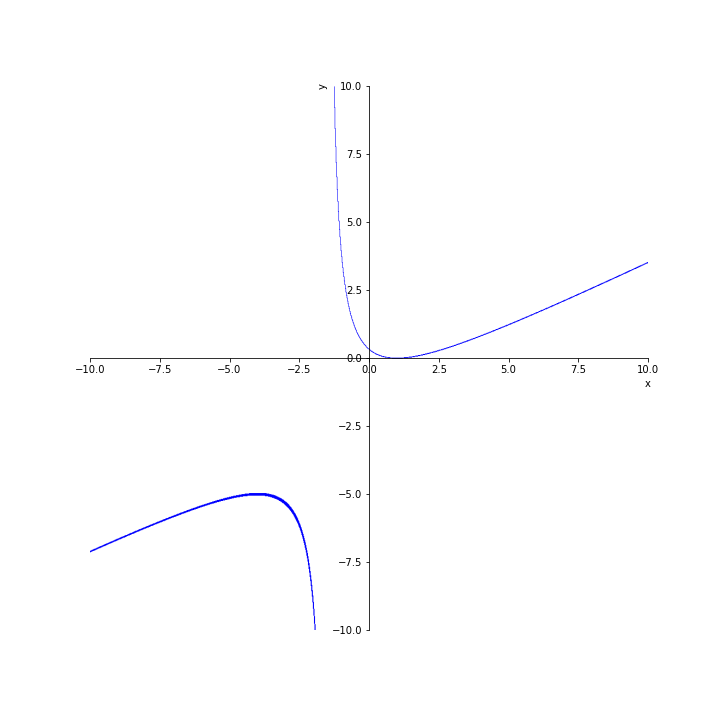
\includegraphics[width=1\columnwidth]{fin301-0}}   \end{solution} \part[2] Asíntotas verticales, horizontales y oblicuas, en caso que existan  \begin{solution}   Asíntotas:\\A.V. $x=-3/2$\\A.O. $y=\frac{x}{2} - \frac{7}{4}$ \\A.O. $y=\frac{x}{2} - \frac{7}{4}$ \\   \end{solution}
%        \end{parts}
%        \end{multicols}


\section*{2ª Evaluación}




  


        % \question[1] Dado el triángulo de vértices A=(-2, -1), \ B=(0, -3),\  y \ C=(2, 1)
        % \begin{multicols}{1}
        % \begin{parts}
        % \part Calcula la recta $\overline{BC}$ \begin{solution}   $6$\   \end{solution} 
        % \part Calcula el área del triángulo \begin{solution}   $6$\   \end{solution}
        %  \end{parts}
        % \end{multicols}
        
                \question[1] Resuelve:
        \begin{multicols}{1}
        \begin{multicols}{2}
        \begin{parts}
        \part $$2\cos^2{x}+\sqrt{3}\cos{x}=0$$ \begin{solution}  90, 150, 210, 270  \end{solution} 
        \part $$\cos{x}=\sen^2{x}-1$$ \begin{solution}   -90, 90  ,180 \end{solution} 
        \part $$2\cos{x}-3\tan{x}=0 $$ \begin{solution}
        $\rightarrow \left [ 150, \quad 30, \quad - \frac{180 i \log{\left (- i \left(- \sqrt{3} + 2\right) \right )}}{\pi}, \quad - \frac{180 i \log{\left (- i \left(\sqrt{3} + 2\right) \right )}}{\pi}\right ]$
        \end{solution}
         \end{parts}
         \end{multicols}
        \end{multicols}
        
        
        \question[1] Dados los vectores $\overrightarrow{a}=(-2, -3)$, $\overrightarrow{b}=(9, -6)$ y $\overrightarrow{c}=(-7, -17)$ expresados en la base canónica:
        \begin{parts}
        \part Demuestra que $B=\left\{\overrightarrow{a},\overrightarrow{b}\right\}$ es una base del plano. ¿Es ortogonal?¿Y ortonormal?
        \begin{solution}
        % Point(-2,-3).dot(Point(9,-6))
        % Point(-2,-3).distance(Point(0,0)
        $\overrightarrow{a}\cdot\overrightarrow{b}=0 \to $ ortogonal y $|\overrightarrow{a}|=\sqrt{13} \to $ no ortonormal
        \end{solution}
        \part Calcula las coordenadas de $\overrightarrow{c}$ respecto de la base $B=\left\{\overrightarrow{a},\overrightarrow{b}\right\}$\begin{solution}
        $(5,\frac{1}{3})$
        \end{solution}
        \end{parts}
        
        \question[1] Dado el triángulo de vértices A=(-2, -1), B=(0, -3) y  C=(2, 1):
        \begin{multicols}{1}
        \begin{parts}
        \part Calcula la longitud de sus lados   \begin{solution}    \end{solution} 
        \part Calcula sus ángulos \begin{solution}   $36'87$ y dos de $71'57$\   \end{solution} 
         \end{parts}
        \end{multicols}
        


        \question[1] \textbf{Ejercicio "Postre":} Si $\sen\alpha=-\frac{5}{13}\land \alpha \in III$ (tercer cuadrante), calcula "sin usar la calculadora":
        \begin{multicols}{4}
        \begin{parts} 
        \part $\cos\alpha$  \begin{solution}   $- \frac{12}{13}$\   \end{solution}
                \part $\tan\alpha$  \begin{solution}   $\frac{5}{12}$\   \end{solution}  
                \part $\cos(\pi+\alpha)$  \begin{solution}   $\frac{12}{13}$\   \end{solution}
                \part $\sen(2\alpha)$  \begin{solution}   $\frac{120}{169}$\   \end{solution} 
        \end{parts}
        \end{multicols}


        % \question Estudia en qué puntos de $\mathbb{R}$ la función no es continua: 
        % \begin{multicols}{1}
        % \begin{parts} \part[2] $f(x)=\begin{cases} \frac{2 x^{2} + 7 x + 3}{x^{2} - 9} & \text{si}\: x \leq -2 \\\frac{\sqrt{x + 3} - 1}{x^{2} + 2 x} & \text{si} \: x > -2\end{cases}$  \begin{solution}   Singularidades de las expresiones analíticas: $\left\{-3, 0\right\}$.\\ Posibles discontinuidades en los extremos de los trozos:-2.\\En -2 no es continua porque no existe límite. Límites laterales: $\frac{3}{5}$ y $- \frac{1}{4}$   \end{solution}
        % \end{parts}
        % \end{multicols}
        
\section*{3ª Evaluación}    

\question[1] Calcula, analíticamente, el área el triángulo de vértices $A(0, -1)$,  $B=(2, 0)$,  y  $C=(1, 1)$.
\begin{solution}
$\frac{3}{2} ud^2$
\end{solution}

\question[1] Luis es saltador de altura, y en el 70\% de sus saltos consigue superar los 2.10 m. Sabiendo que en una competición tiene que saltar tres veces, halla la probabilidad de que:
\begin{multicols}{2}

\begin{parts} 
\part  En todas supere los 2.10 m.  \begin{solution}  $ 0.3430$  \end{solution} 
\part  No los supere en ninguna  \begin{solution}  $0.02700 $  \end{solution}
\part  Si su primer salto fue nulo, supere los 2.10 m en, al menos, una ocasión.  \begin{solution}  $0.9100$  \end{solution}
        \end{parts}
\end{multicols}        
        
    
        \question[1] Calcula los siguientes límites: 
        \begin{multicols}{2}
        \begin{parts} \part $$\lim_{x \to -1}\left(\frac{x^{2} - 1}{x^{2} + 3 x + 2}\right)$$  \begin{solution}   $-2$ \end{solution}
        % \part $$\lim_{x \to \infty}\left(- x + \sqrt{x^{2} + x + 1}\right)$$  \begin{solution}   $\frac{1}{2}$ \end{solution}
         
         \part $$\lim_{x \to 1}\left( \frac{1}{1 - x}- \frac{3}{1 - x^{2}}\right)$$\begin{solution}
         No existe
         \end{solution}
         
         
        \end{parts}
        \end{multicols}
        
%        \question Halla a y b de modo que las siguientes funciones sean continuas:
%        \begin{multicols}{1}
%        \begin{parts} \part[2] $$f(x)=\begin{cases} a + e^{x + 2} & \text{si}\: x \leq -2 \\\frac{x + 1}{3 - x} & \text{si}\: -2 < x < 1 \\b x + 3 & \text{si}\: x \geq 1 \end{cases}$$  \begin{solution}   $\left\{ a : - \frac{6}{5}, \  b : -2\right\}$   \end{solution}
%        \end{parts}
%        \end{multicols}
        
%        \question Halla a y b de modo que las siguientes funciones sean continuas:
%        \begin{multicols}{1}
%        \begin{parts} \part[2] $$f(x)=\begin{cases} a + e^{x + 3} & \text{si}\: x \leq -3 \\\frac{x + 2}{4 - x} & \text{si}\: -3 < x < 1 \\b x + 6 & \text{si}\: x \geq 1 \end{cases}$$  \begin{solution}   $\left\{ a : - \frac{8}{7}, \  b : -5\right\}$   \end{solution}
%        \end{parts}
%        \end{multicols}
        
        %         \question[1] Dada la función:$$f(x)=\frac{- x^{2} - x + 3}{x^{2} + x - 2}$$, calcular:
        % \begin{multicols}{1}
        % \begin{parts} \part Dominio de $f(x)$  \begin{solution}   $Dom(f)=\left(-\infty, -2\right) \cup \left(-2, 1\right) \cup \left(1, \infty\right)$\\  \end{solution} \part Asíntotas verticales, horizontales y oblicuas, en caso que existan  \begin{solution}   Asíntotas:\\A.V. $x=-2$\\, A.V. $x=1$\\A.H. $y=-1$\\A.H. $y=-1$\\A.O. $y=-1$ \\A.O. $y=-1$ \\   \end{solution}
        % \end{parts}
        % \end{multicols}
        
        
        
%        \question Deriva las siguientes funciones (simplificando el resultado al máximo):
%        \begin{multicols}{1}
%        \begin{parts} \part[1] $y=\frac{3 x^{2} - 2 x + 1}{\left(x - 1\right)^{2}}$  \begin{solution}   $y'=- \frac{4 x}{x^{3} - 3 x^{2} + 3 x - 1}$   \end{solution} \part[1] $y=\sqrt{\sqrt{x} + 1}$  \begin{solution}   $y'=\frac{1}{4 \sqrt{x} \sqrt{\sqrt{x} + 1}}$   \end{solution} \part[1] $y=\frac{\log{\left(x^{2} \right)}}{x}$  \begin{solution}   $y'=\frac{2 - \log{\left(x^{2} \right)}}{x^{2}}$   \end{solution} \part[1] $y=3 \sin{\left(\cos{\left(2 x \right)} \right)}$  \begin{solution}   $y'=- 6 \sin{\left(2 x \right)} \cos{\left(\cos{\left(2 x \right)} \right)}$   \end{solution}
%        \end{parts}
%        \end{multicols}
        
%        \question Deriva las siguientes funciones:
%        \begin{multicols}{1}
%        \begin{parts} \part[1] $y=\frac{2 x^{2} - 2 x + 1}{\left(x - 1\right)^{2}}$  \begin{solution}   $y'=- \frac{2 x}{x^{3} - 3 x^{2} + 3 x - 1}$   \end{solution} \part[1] $y=\sqrt{2 - \sqrt{x}}$  \begin{solution}   $y'=- \frac{1}{4 \sqrt{x} \sqrt{2 - \sqrt{x}}}$   \end{solution} \part[1] $y=\frac{\ln{\left(x \right)}}{x}$  \begin{solution}   $y'=\frac{1 - \ln{\left(x \right)}}{x^{2}}$   \end{solution} \part[1] $y=2 \cos{\left(\sin{\left(2 x \right)} \right)}$  \begin{solution}   $y'=- 4 \sin{\left(\sin{\left(2 x \right)} \right)} \cos{\left(2 x \right)}$   \end{solution}
%        \end{parts}
%        \end{multicols}
        
%        \question Se dispone de dos cajas, la caja A contiene 3 bolas moradas y 2 bolas rojas; mientras que la caja B contiene 4
%    bolas moradas y 4 rojas.
%        \begin{multicols}{1}
%        \begin{parts} \part[2] Se escoge una bola cualquiera de la caja A y se pasa a la caja B. Posteriormente se saca una
%    bola de la caja B. ¿Cuál es la probabilidad de que la bola extraída de la caja B sea morada?.   \begin{solution}   $\frac{3}{5}\cdot\frac{5}{9}+\frac{2}{5}\cdot\frac{4}{9}=\frac{23}{45}$   \end{solution} \part[2] Ahora volvemos a la situación original de las cajas. Seleccionamos una caja al azar y se saca una bola 
%    que resulta ser roja. ¿Cuál es la probabilidad de que esa
%    bola sea de la caja A?  \begin{solution}   $\dfrac{\frac{1}{2}\cdot\frac{2}{5}}{\frac{1}{2}\cdot\frac{2}{5}+\frac{1}{2}\cdot\frac{1}{2}}=\frac{4}{9}$   \end{solution}
%        \end{parts}
%        \end{multicols}
%        \question Se dispone de dos cajas, la caja A contiene 3 bolas verdes y 2 bolas blancas; mientras que la caja B contiene 4
%    bolas verdes y 4 blancas.
%        \begin{multicols}{1}
%        \begin{parts} \part[2] Se escoge una bola cualquiera de la caja A y se pasa a la caja B. Posteriormente se saca una
%    bola de la caja B. ¿Cuál es la probabilidad de que la bola extraída de la caja B sea verde?.   \begin{solution}   $\frac{3}{4}\cdot\frac{5}{9}+\frac{1}{4}\cdot\frac{4}{9}=\frac{19}{36}$   \end{solution} \part[2] Ahora volvemos a la situación original de las cajas. Seleccionamos una caja al azar y se saca una bola 
%    que resulta ser blanca. ¿Cuál es la probabilidad de que esa
%    bola sea de la caja A?  \begin{solution}   $\dfrac{\frac{1}{2}\cdot\frac{1}{4}}{\frac{1}{2}\cdot\frac{1}{4}+\frac{1}{2}\cdot\frac{1}{2}}=\frac{1}{3}$   \end{solution}
%        \end{parts}
%        \end{multicols}


\question[1] \textbf{Ejercicio "postre":} En una bolsa, A, hay 2 bolas negras y 3 rojas. En otra bolsa, B, hay 3 bolas negras, 4 rojas y 3 verdes. Extraemos una bola de A y la introducimos en la bolsa B. Posteriormente, sacamos una bola de B:
%\noaddpoints % to omit double points count

\begin{parts}
\part ¿Cuál es la probabilidad de que la segunda bola sea roja?
\begin{solution}
$\frac{8}{55}+\frac{2}{11}=\frac{23}{55}$ 
\end{solution}
\part ¿Cuál es la probabilidad de que las dos bolas extraídas sean rojas?
\begin{solution}
$\frac{3}{11}$
\end{solution}
\part ¿Cuál es la probabilidad de que la primera haya sido negra si sabemos que la segunda ha sido roja?
\begin{solution}
$\frac{\frac{8}{55}}{\frac{23}{55}}=\frac{8}{23}$
\end{solution}
\end{parts}

% \question \textbf{Ejercicio "postre":} La temperatura media en los meses de invierno en varias ciudades y el gasto medio por habitante en
% calefacción ha sido:\\
% \\
% \begin{tabular}{|c||c|c|c|c|c|c|}
% \hline 
% Temperatura (ºC) & 10 & 12 & 14 & 16  \\ 
% \hline 
% Gasto (\euro ) & 150 & 120 & 102 & 90  \\ 
% \hline 
% \end{tabular} \\
% \begin{parts}
% \part Halla el coeficiente de correlación lineal 
% \begin{solution}
% \begin{tabular}{rrrrrr}
% \hline
%     &   x &     y &   xy &   x2 &    y2 \\
% \hline
%   0 &  10 & 150   & 1500 &  100 & 22500 \\
%   1 &  12 & 120   & 1440 &  144 & 14400 \\
%   2 &  14 & 102   & 1428 &  196 & 10404 \\
%   3 &  16 &  90   & 1440 &  256 &  8100 \\
%   \hline
%   4 &  52 & 462   & 5808 &  696 & 55404 \\
%   \hline
%   5 &  13 & 115.5 & 1452 &  174 & 13851 \\
% \hline
% \end{tabular}
% \\

% covarianza	-49.5 \\
% desvx	2.23606797749979 \\
% desvy	22.599778759979046 \\
% coefcorr -0.9795260923726159 \\
% \end{solution}
% \part Estima, razonadamente, el gasto medio por habitante de una ciudad si la temperatura media hubiera sido de 11ºC. ¿Es fiable la estimación obtenida? 

% \begin{solution}
% $y = -9.9x + 244.2$ \\ Valor estimado para 11: 135.3 \euro 
% \end{solution}
% \end{parts}




        
    \end{questions}
    \end{document}
    
